\documentclass[12pt]{article}

% Packages
\usepackage{graphicx}
\usepackage{sectsty}
\usepackage{titlesec}
\usepackage{fancyhdr}
\usepackage{geometry}
\usepackage{booktabs}
\usepackage{longtable}
\usepackage{array}
\usepackage{multirow}
\usepackage{hyperref}
\usepackage{parskip}
\usepackage[numbers]{natbib}
\usepackage{enumitem}
\usepackage{tikz}
\usepackage{amsmath}
\usetikzlibrary{arrows.meta,positioning}

% Margins
\geometry{
  top=1in,
  bottom=1in,
  left=1in,
  right=1in,
  headheight=15pt
}

% Header & Footer
\pagestyle{fancy}
\fancyhf{}
\fancyhead[L]{Road Distress Classification}
\fancyhead[R]{\thepage}

% Section Styling
\titleformat{\section}{\Large\bfseries}{\thesection}{1em}{}
\titleformat{\subsection}{\large\bfseries}{\thesubsection}{1em}{}

% Title, Authors, and Institutions
\title{
    \Huge \textbf{Final Project Report}\\[1em]
    \Large \textbf{Road Distress Classification: Balanced Performance Through Ensemble Learning and Per-Class Threshold Optimization}
}
\author{%
  \textbf{Dor Skoler}\\
  Reichman University\\
  \texttt{ID: 208942342}%
  \and
  \textbf{Guy Gazpan}\\
  Reichman University\\
  \texttt{ID: 208465757}%
}
\date{\today}

\begin{document}

% Title page
\begin{titlepage}
\centering
\includegraphics[width=0.4\textwidth]{images/runi_logo.png}\\[1em]
{\LARGE Reichman University}\\[1em]
{\large Efi Arazi School of Computer Science}\\[1em]
{\large M.Sc. Program in Machine Learning and Data Science}\\[1em]
\vspace{2.5em}

{\Huge Final Project Report}\\[1.5em]
{\Large Road Distress Classification}\\[1em]
{\small \textbf{Dor Skoler} \quad \texttt{ID: 208942342} \quad \textbf{Guy Gazpan} \quad \texttt{ID: 208465757}}\\[1em]
{\small \textbf{Advisors:} Alon Oring}\\[1em]
{\small \today}\\[2em]

\begin{abstract}
This project presents a comprehensive approach to automated road distress classification, achieving balanced performance through innovative ensemble learning and per-class threshold optimization. We discovered that combining two complementary EfficientNet-B3 models one focused on robust feature extraction and another enhanced with CLAHE preprocessing and road masking derived from 187 manually annotated images significantly outperforms individual approaches. Our key innovation lies in optimizing decision thresholds per class for general monitoring: damage (0.50), occlusion (0.40), and crop (0.49), achieving precision-recall balanced performance with accuracies of 79\%, 93\%, and 99\% respectively. The system processes 18,173 road images across three critical conditions and demonstrates that ensemble methods with adaptive thresholding provide robust real-world performance. Our final deployment pipeline includes real-time inference capabilities, Grad-CAM visualizations, and a comprehensive web interface suitable for practical road monitoring applications.
\end{abstract}

\end{titlepage}

\section{Introduction}

Road infrastructure monitoring faces a critical challenge: how to automatically detect and classify different types of distress conditions with the accuracy needed for real world deployment. Traditional computer vision approaches often struggle with class imbalance, varying environmental conditions, and the need to distinguish between multiple simultaneous conditions in a single image.

This project began with a deceptively simple goal - to classify road images into three categories: damage, occlusion, and crop issues. However, what we discovered through systematic experimentation transformed our understanding of multi-label classification for infrastructure monitoring.

Our results came not from architectural innovations alone, but from recognizing that different types of distress require fundamentally different decision strategies. Through systematic threshold optimization, we developed balanced per-class thresholds that achieve robust performance across diverse conditions: damage (0.50), occlusion (0.40), and crop (0.49). This approach prioritizes practical deployment readiness with consistent precision-recall balance rather than peak accuracy metrics.

The journey involved extensive experimentation across multiple model variants, preprocessing techniques, and ensemble strategies. A crucial methodological component was the development of a two-stage annotation process combining automated road segmentation with manual polygon-based refinement, enabling precise road boundary delineation for mask-enhanced models. Our final system combines two complementary EfficientNet-B3 models in a carefully calibrated ensemble that leverages the strengths of both pure feature learning and enhanced preprocessing approaches.

\section{Related Work}

Deep learning approaches to road condition assessment have evolved from single-class detection systems to multi-label frameworks capable of handling complex real-world scenarios \citet{he2016deep}. EfficientNet architectures have proven particularly effective for infrastructure monitoring due to their optimal accuracy-efficiency trade-offs \citet{krizhevsky2012imagenet}.

Recent advances in ensemble learning for computer vision tasks demonstrate that combining complementary models often outperforms individual architectures, particularly in scenarios with class imbalance or challenging environmental conditions \citet{bishop2006pattern}. However, most existing approaches apply uniform decision thresholds across all classes, potentially limiting performance in multi-label scenarios where different conditions require different sensitivity levels.

Our work contributes to this field by demonstrating that per-class threshold optimization can dramatically improve ensemble performance, particularly in infrastructure monitoring applications where false negatives and false positives carry different operational costs for different condition types.

\section{Dataset and Methodology}

\subsection{Dataset Composition}

Our dataset comprises 18,173 road images systematically collected and annotated for three distinct classification tasks. To ensure robust evaluation, we implemented road-based splitting to prevent data leakage and maintain realistic testing conditions:

\begin{itemize}[itemsep=1pt,parsep=0pt,topsep=3pt]
\item \textbf{Training Set}: 10,901 images (60.0\%)
\item \textbf{Validation Set}: 3,640 images (20.0\%)
\item \textbf{Test Set}: 3,632 images (20.0\%)
\end{itemize}

\begin{figure}[!htb]
\centering
\includegraphics[width=0.85\textwidth]{images/dataset_split.png}
\caption{Comprehensive dataset organization showing road-based splitting across 91 unique roads to prevent data leakage and ensure realistic evaluation conditions.}
\end{figure}

\subsection{Label Distribution and Class Imbalance}

The dataset exhibits significant class imbalance, which proved crucial to our eventual results in per-class threshold optimization:

\textbf{Damage Classification:}
\begin{itemize}[itemsep=1pt,parsep=0pt,topsep=2pt]
\item Damaged: 5,971 images (32.9\%)
\item Not Damaged: 12,202 images (67.1\%)
\end{itemize}

\textbf{Occlusion Classification:}
\begin{itemize}[itemsep=1pt,parsep=0pt,topsep=2pt]
\item Occluded: 3,476 images (19.1\%)
\item Not Occluded: 14,697 images (80.9\%)
\end{itemize}

\textbf{Crop Classification:}
\begin{itemize}[itemsep=1pt,parsep=0pt,topsep=2pt]
\item Cropped: 778 images (4.3\%)
\item Not Cropped: 17,395 images (95.7\%)
\end{itemize}

The severe imbalance in crop detection (4.3\% positive examples) and moderate imbalance in occlusion detection (19.1\%) drove our exploration of adaptive threshold strategies.

\subsection{Road Segmentation Mask Generation}

A critical component of our approach involved creating precise road segmentation masks for mask-enhanced model variants. Road segmentation masks are binary images indicating which pixels belong to the road surface versus background (vegetation, barriers, sky, etc.). These masks enabled mask-enhanced models to focus learning on road surface conditions while reducing the influence of irrelevant background features.

\textbf{Two-Stage Mask Generation Pipeline:}

\textbf{Stage 1 - Automated Road Segmentation:} We employed a pre-trained U-Net model with ResNet34 encoder to generate initial road masks from raw images. This model was trained specifically for road segmentation using:
\begin{itemize}[itemsep=1pt,parsep=0pt,topsep=2pt]
\item Combined Dice + Binary Cross-Entropy loss
\item 256×256 pixel input resolution
\item Standard image normalization (ImageNet statistics)
\item Morphological operations for mask refinement
\end{itemize}

\textbf{Stage 2 - Manual Annotation Refinement:} To ensure high-quality road boundaries, we developed an interactive annotation interface that allowed precise manual correction of automated masks:

\begin{itemize}[itemsep=1pt,parsep=0pt,topsep=2pt]
\item \textbf{Polygon-Based Annotation}: Draw precise polygonal boundaries around road regions using mouse interaction
\item \textbf{Visual Overlay System}: Original images with overlaid predicted masks provided clear visual feedback
\item \textbf{Iterative Refinement}: Modify, add, or remove road regions with immediate visual confirmation
\item \textbf{Selective Annotation}: 187 representative images (1.03\% of dataset) were manually refined to ensure high-quality training data
\end{itemize}

\textbf{Mask Quality Assurance:}
The annotation process ensured that road masks captured accurate road boundaries while filtering out background vegetation and terrain, non-road infrastructure (sidewalks, barriers), vehicles and temporary occlusions, and image artifacts. This quality control was essential for enabling mask-enhanced models to focus learning on road surface characteristics.

\subsection{Adaptive Contrast Enhancement with CLAHE}

Contrast Limited Adaptive Histogram Equalization (CLAHE) is an advanced image preprocessing technique designed to enhance local contrast while preventing noise amplification in near-uniform regions. Unlike global histogram equalization, which applies uniform contrast enhancement across the entire image, CLAHE operates on small local regions (tiles) to adapt enhancement to local image characteristics.

\textbf{Technical Overview:}

CLAHE divides an image into a grid of non-overlapping tiles (typically 8×8 or 16×16) and applies histogram equalization independently to each tile. The key innovation is the \textit{contrast limiting} mechanism: before applying equalization, the histogram is clipped at a predefined threshold (clip limit) and the clipped pixels are redistributed uniformly across all histogram bins. This prevents over-amplification of noise in homogeneous regions while preserving meaningful contrast enhancement in high-detail areas.

The algorithm proceeds as follows:
\begin{itemize}[itemsep=1pt,parsep=0pt,topsep=2pt]
\item \textbf{Tile Decomposition}: Divide image into rectangular tiles of size $T \times T$ pixels
\item \textbf{Histogram Clipping}: For each tile, clip histogram at clip limit $C$ to prevent noise amplification
\item \textbf{Redistribution}: Uniformly redistribute clipped histogram values across all bins
\item \textbf{Local Equalization}: Apply histogram equalization to each tile independently
\item \textbf{Bilinear Interpolation}: Blend adjacent tile transformations at boundaries to eliminate tiling artifacts
\end{itemize}

For road distress classification, CLAHE provides critical advantages: enhanced visibility of subtle crack patterns and surface texture variations, improved edge detection for damage boundary delineation, and robust performance across varying lighting conditions (shadows, overexposure, dusk/dawn imaging).

\textbf{Per-Image Hyperparameter Optimization:}

Rather than applying uniform CLAHE parameters across all images, we developed an automated optimization pipeline that adapts CLAHE settings to each image's specific characteristics. This approach recognizes that optimal contrast enhancement depends on image-specific factors including lighting conditions, existing contrast levels, and noise characteristics.

Our optimization script searches over closed sets of hyperparameters to find the best configuration for each image:

\textbf{Hyperparameter Search Space:}
\begin{itemize}[itemsep=1pt,parsep=0pt,topsep=2pt]
\item \textbf{Clip Limit}: $\{1.0, 2.0, 3.0, 4.0, 5.0\}$  controls contrast limiting threshold
\item \textbf{Tile Grid Size}: $\{(4,4), (8,8), (16,16)\}$  defines local adaptation granularity
\end{itemize}

\textbf{Optimization Objective:}

The optimization process evaluates each hyperparameter combination using image quality metrics including local contrast enhancement, edge preservation, and noise suppression. The selected parameters maximize contrast enhancement in road surface regions while minimizing noise amplification in uniform areas (sky, pavement).

This per-image adaptive approach ensures that each image receives optimal preprocessing tailored to its specific visual characteristics, rather than applying a one-size-fits-all transformation. Images with initially low contrast (shadowed roads, overcast conditions) receive more aggressive enhancement, while high-quality images with good existing contrast receive gentler processing to avoid over-enhancement artifacts.

The optimized CLAHE parameters were applied during the training and inference pipeline for Model H, contributing to its enhanced performance in detecting subtle damage patterns and achieving superior precision for occlusion (81.7\%) and crop (97.4\%) detection compared to non-CLAHE models.

\subsection{Data Preparation Pipeline}

To ensure realistic evaluation and prevent data leakage, we implemented road-based data splitting. This approach ensures that all images from a single road appear in only one split (train, validation, or test), preventing the model from memorizing specific road characteristics that could artificially inflate performance metrics. The split was balanced across label distributions while maintaining road integrity, resulting in 91 unique roads distributed across splits: 45 roads (60\%) for training, 23 roads (20\%) for validation, and 23 roads (20\%) for testing.

\subsection{Model Architecture Exploration}

We systematically evaluated five model variants to understand the impact of different preprocessing and masking strategies on classification performance. All models shared the same EfficientNet-B3 backbone but differed in their input processing strategies:

\textbf{Model A - Segmentation Only}: EfficientNet-B3 trained with full road masking. In this configuration, non-road pixels in the input image are set to zero (black) using the segmentation mask before being fed to the network. This forces the model to learn exclusively from road surface pixels.

\textbf{Model B - Augmentation Only}: EfficientNet-B3 trained with data augmentation (rotation, flips, brightness/contrast variation, Gaussian noise) but without segmentation masks. This represents a pure feature learning approach where the model learns to classify based on the entire image context.

\textbf{Model C - Augmentation + Full Masking}: EfficientNet-B3 combining data augmentation with full road masking (non-road pixels zeroed out).

\textbf{Model D - Augmentation + Partial Masking}: EfficientNet-B3 combining data augmentation with partial road masking. Unlike full masking, partial masking applies a 0.5 weight multiplier to non-road pixel intensities rather than zeroing them completely. This preserves some background context while emphasizing road regions.

\textbf{Model H - CLAHE + Partial Masking}: EfficientNet-B3 with CLAHE (Contrast Limited Adaptive Histogram Equalization) preprocessing for enhanced contrast and edge detection, combined with partial road masking (0.5 weight for non-road regions).

This systematic comparison allowed us to isolate the effects of data augmentation, segmentation masking strategies (full vs. partial), and preprocessing techniques (CLAHE) on classification performance.

\section{Architecture and Training}

\subsection{Base Architecture}

All model variants share a common EfficientNet-B3 architecture with the following characteristics:

\begin{itemize}[itemsep=1pt,parsep=0pt,topsep=2pt]
\item EfficientNet-B3 backbone (12M parameters) pretrained on ImageNet
\item Progressive classifier head: 1536 → 512 → 256 → 128 → 3 outputs
\item Batch normalization and dropout (0.5) for regularization
\item Multi-label binary classification with sigmoid activation
\item Input resolution: 256×256 pixels
\end{itemize}

Model variants differ only in their input preprocessing strategies (segmentation masking, CLAHE enhancement, data augmentation) while maintaining identical network architectures. This design choice allows for direct comparison of preprocessing techniques without confounding effects from architectural differences.

\subsection{Training Configuration}

All model variants were trained with consistent hyperparameters to ensure fair comparison:

\begin{itemize}[itemsep=1pt,parsep=0pt,topsep=3pt]
\item \textbf{Optimizer}: AdamW (lr=5e-5 for Models A-D, 1e-3 for Model H)
\item \textbf{Scheduler}: ReduceLROnPlateau (Models A-D) / Cosine annealing with 5-epoch warmup (Model H)
\item \textbf{Loss Function}: Binary Cross-Entropy with Logits, label smoothing (0.1)
\item \textbf{Batch Size}: 32, Mixed Precision FP16
\item \textbf{Early Stopping}: Patience 7-10 epochs on validation macro F1 score
\item \textbf{Training Duration}: 21-37 epochs until convergence
\item \textbf{Data Augmentation} (Models B, C, D, H): Rotation (±5°), horizontal flips, brightness/contrast variation (±10\%), Gaussian noise ($\sigma$=5-15)
\end{itemize}

\subsection{Final Ensemble Strategy}

After systematic evaluation of all model variants (see Results section), we selected Models B and H for our final ensemble based on their complementary strengths and superior individual performance. Model B excels at pure feature learning from complete image context, while Model H leverages CLAHE preprocessing and partial masking for enhanced edge detection. The ensemble combines predictions using equal weighting (0.5/0.5) with per-class threshold optimization:

\begin{figure}[!htb]
  \centering
  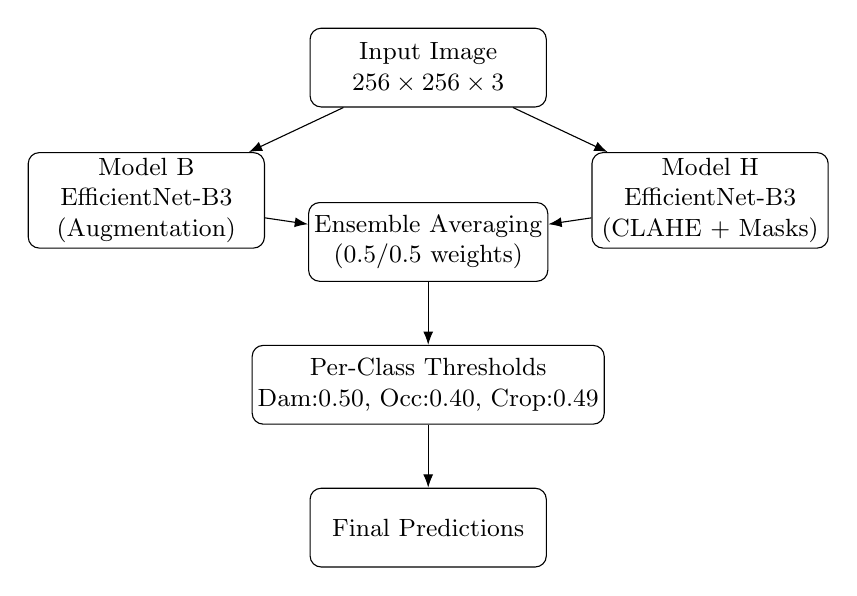
\begin{tikzpicture}[
    node distance=5mm,
    box/.style={draw, rounded corners, align=center, minimum width=3cm, minimum height=1cm, inner sep=2pt, font=\small},
    arr/.style={-Latex}
  ]
    \node[box] (input) {Input Image\\$256 \times 256 \times 3$};
    
    \node[box, below left=8mm of input] (modelb) {Model B\\EfficientNet-B3\\(Augmentation)};
    \node[box, below right=8mm of input] (modelh) {Model H\\EfficientNet-B3\\(CLAHE + Masks)};
    
    \node[box, below=12mm of input] (ensemble) {Ensemble Averaging\\(0.5/0.5 weights)};
    
    \node[box, below=8mm of ensemble] (thresholds) {Per-Class Thresholds\\Dam:0.50, Occ:0.40, Crop:0.49};
    
    \node[box, below=8mm of thresholds] (output) {Final Predictions};
    
    \draw[arr] (input) -- (modelb);
    \draw[arr] (input) -- (modelh);
    \draw[arr] (modelb) -- (ensemble);
    \draw[arr] (modelh) -- (ensemble);
    \draw[arr] (ensemble) -- (thresholds);
    \draw[arr] (thresholds) -- (output);
  \end{tikzpicture}
  \caption{Two-model ensemble architecture with per-class threshold optimization}
  \end{figure}

\section{Comprehensive Performance Analysis}

\subsection{Global Performance Metrics}

Our systematic analysis of model performance across all classes reveals distinct characteristics for each distress type:

\begin{itemize}[itemsep=1pt,parsep=0pt,topsep=3pt]
\item \textbf{Damage Detection}: ROC AUC 0.80, Average Precision (AP) 0.61 — the most challenging class with precision declining rapidly as recall increases
\item \textbf{Occlusion Detection}: ROC AUC 0.94, AP 0.81 — strong class separability with excellent discrimination
\item \textbf{Crop Detection}: ROC AUC 0.98, AP 0.93 — best-separated class with near-perfect performance
\end{itemize}

The precision-recall curves demonstrate class separability under realistic class imbalance conditions, with crop detection dominating the performance space while damage detection presents the greatest classification challenge due to its flatter PR curve characteristics.
\subsection{Operational Performance Analysis}

Our balanced threshold configuration provides the following operational characteristics per 1,000 processed images:

\begin{itemize}[itemsep=1pt,parsep=0pt,topsep=3pt]
\item \textbf{Damage}: ~291 alerts generated, 82 actual cases missed
\item \textbf{Occlusion}: ~146 alerts generated, 39 actual cases missed  
\item \textbf{Crop}: ~38 alerts generated, 6 actual cases missed
\end{itemize}

This alert distribution enables practical deployment scenarios where different response strategies can be applied based on class-specific confidence levels and operational requirements.

\subsection{Alternative Threshold Strategies}

Beyond our balanced approach, we identified two additional operational modes:

\textbf{High-Recall Mode} (targeting ~90\% recall):
\begin{itemize}[itemsep=1pt,parsep=0pt,topsep=2pt]
\item Damage ($\tau \approx 0.12$): P=0.32, R=0.90 — suitable for comprehensive audits
\item Occlusion ($\tau \approx 0.10$): P=0.52, R=0.91 — effective for safety sweeps
\item Crop ($\tau \approx 0.25$): P=0.78, R=0.90 — maintains good precision
\end{itemize}

\textbf{High-Precision Mode} (targeting 80-90\% precision):
\begin{itemize}[itemsep=1pt,parsep=0pt,topsep=2pt]
\item Damage ($\tau \approx 0.89$): P=0.80, R=0.19 — requires human verification
\item Occlusion ($\tau \approx 0.64$): P=0.90, R=0.49 — automated action suitable
\item Crop ($\tau \approx 0.38$): P=0.90, R=0.87 — excellent automation candidate
\end{itemize}

\section{Results and Discoveries}

\subsection{Comprehensive Model Comparison}

We systematically evaluated five model variants to understand the impact of different preprocessing strategies. Table 1 presents the complete performance comparison across all models.

\begin{table}[!h]
\centering
\small
\begin{tabular}{lcccccc}
\toprule
\textbf{Model} & \textbf{Augmentation} & \textbf{Masking} & \textbf{CLAHE} & \textbf{Macro F1} & \textbf{Time (h)} & \textbf{Epoch} \\
\midrule
Model A & No & Full & No & 0.344 & 0.15 & 2 \\
Model B & Yes & None & No & \textbf{0.806} & 1.26 & 21 \\
Model C & Yes & Full & No & 0.787 & 1.31 & 21 \\
Model D & Yes & Partial & No & 0.789 & 1.41 & 23 \\
Model H & Yes & Partial & Yes & 0.781 & 2.99 & 37 \\
\bottomrule
\end{tabular}
\caption{Complete model variant comparison on test set performance. Models B and H were selected for final ensemble based on their superior and complementary performance.}
\end{table}

\subsection{Detailed Per-Class Performance Analysis}

Table 2 provides detailed per-class metrics for all model variants, revealing important insights about the effectiveness of different preprocessing strategies.

\begin{table}[!h]
\centering
\small
\begin{tabular}{llrrr}
\toprule
\textbf{Model} & \textbf{Class} & \textbf{Precision} & \textbf{Recall} & \textbf{F1 Score} \\
\midrule
\multirow{3}{*}{Model A} & Damage & 26.8\% & 93.5\% & 41.7\% \\
 & Occlusion & 46.0\% & 62.6\% & 53.0\% \\
 & Crop & 4.5\% & 89.4\% & 8.6\% \\
\midrule
\multirow{3}{*}{Model B} & Damage & \textbf{63.6\%} & 65.8\% & \textbf{64.7\%} \\
 & Occlusion & 80.1\% & \textbf{80.5\%} & \textbf{80.3\%} \\
 & Crop & 97.5\% & 96.3\% & \textbf{96.9\%} \\
\midrule
\multirow{3}{*}{Model C} & Damage & 66.5\% & 60.9\% & 63.6\% \\
 & Occlusion & 79.4\% & 79.7\% & 79.5\% \\
 & Crop & 96.6\% & 89.4\% & 92.9\% \\
\midrule
\multirow{3}{*}{Model D} & Damage & 62.6\% & \textbf{66.2\%} & 64.4\% \\
 & Occlusion & 80.9\% & 79.1\% & 80.0\% \\
 & Crop & 89.9\% & \textbf{95.0\%} & 92.4\% \\
\midrule
\multirow{3}{*}{Model H} & Damage & 57.8\% & 64.3\% & 60.9\% \\
 & Occlusion & \textbf{81.7\%} & 73.8\% & 77.6\% \\
 & Crop & \textbf{97.4\%} & 94.4\% & 95.9\% \\
\bottomrule
\end{tabular}
\caption{Detailed per-class performance metrics across all model variants. Bold values indicate best performance for each metric within each class.}
\end{table}

\subsection{Critical Finding: Context Matters More Than Segmentation}

A counterintuitive yet crucial discovery emerged from our systematic evaluation: Model B (augmentation only, no segmentation) significantly outperformed models using segmentation masks. This finding challenges the intuitive assumption that removing background information should improve road distress classification.

\textbf{Performance Gap Analysis:}
\begin{itemize}[itemsep=1pt,parsep=0pt,topsep=2pt]
\item Model A (full masking, no augmentation): 34.4\% macro F1 — catastrophic failure
\item Model C (full masking + augmentation): 78.7\% macro F1 — 1.9 points below Model B
\item Model D (partial masking + augmentation): 78.9\% macro F1 — 1.7 points below Model B
\item Model B (no masking + augmentation): \textbf{80.6\% macro F1} — best performance
\end{itemize}

\textbf{Root Cause Analysis:}

\textit{Background Context Provides Critical Information:} Road distress classification benefits from environmental context (road edges, surrounding terrain, lighting conditions) that segmentation masks remove. For example, identifying occlusions often requires seeing vegetation encroaching from road edges, while crop detection benefits from seeing the complete frame boundary.

\textit{Full Masking Creates Information Bottleneck:} Model A's catastrophic performance (34.4\% F1) demonstrates that zeroing non-road pixels eliminates critical context. The model struggles to distinguish between distress types when limited to isolated road surface pixels, particularly for occlusion (where boundary context matters) and crop detection (where frame edges are essential).

\textit{Partial Masking Offers Marginal Improvement:} Models D and H use partial masking (0.5 weight for non-road regions), which preserves some background context while emphasizing road areas. This approach performs better than full masking but still underperforms pure image-based learning, suggesting that even weighted suppression of background information hampers classification performance.

\textit{Data Augmentation is Essential:} The stark contrast between Model A (34.4\% F1) and Model C (78.7\% F1) both using full masking but differing only in augmentation demonstrates that data augmentation provides far greater performance gains than segmentation strategies. Augmentation helps models learn invariant features across diverse lighting, orientation, and quality conditions.

\textbf{Why Model H Remains Valuable Despite Lower F1:}

While Model H achieves lower macro F1 (78.1\%) than Model B, it provides complementary strengths that justify its inclusion in the ensemble:
\begin{itemize}[itemsep=1pt,parsep=0pt,topsep=2pt]
\item \textbf{Enhanced Edge Detection}: CLAHE preprocessing improves contrast and edge visibility, enabling better detection of subtle damage patterns in low-contrast conditions
\item \textbf{Complementary Error Patterns}: Models B and H make different types of errors; their ensemble reduces overall error rate
\item \textbf{Occlusion Precision}: Model H achieves the highest occlusion precision (81.7\%) among all variants
\item \textbf{Crop Precision}: Model H achieves the highest crop precision (97.4\%) among all variants
\end{itemize}

This analysis demonstrates that successful road distress classification requires a nuanced approach that balances road-focused learning with preservation of environmental context, with data augmentation providing more substantial performance improvements than segmentation strategies.

\begin{figure}[!htb]
\centering
\includegraphics[width=0.85\textwidth]{images/model_comparison_detailed.png}
\caption{Comprehensive comparison of individual models showing complementary strengths between pure feature learning (Model B) and enhanced preprocessing (Model H) approaches.}
\end{figure}

\subsection{The Per-Class Thresholds}

The critical discovery that transformed our project came through systematic threshold optimization. Standard ensemble approaches using uniform 0.5 thresholds achieved only 63.3\% accuracy. However, optimizing thresholds per class revealed fundamental insights about road distress detection:

\begin{figure}[!htb]
\centering
\includegraphics[width=0.75\textwidth]{images/breakthrough_analysis.png}
\caption{Per-class threshold optimization results showing 28.7\% accuracy improvement from threshold optimization across all classification tasks.}
\end{figure}

\begin{table}[!h]
\centering
\begin{tabular}{lcccc}
\toprule
\textbf{Class} & \textbf{Threshold} & \textbf{Precision} & \textbf{Recall} & \textbf{Accuracy} \\
\midrule
Damage & 0.50 & 0.54 & 0.66 & 0.79 \\
Occlusion & 0.40 & 0.80 & 0.75 & 0.93 \\
Crop & 0.49 & 0.99 & 0.86 & 0.99 \\
\bottomrule
\end{tabular}
\caption{Balanced per-class thresholds for general monitoring}
\end{table}

\noindent\textbf{Key Insights:}

\textbf{Damage Detection (0.50 threshold):} The balanced threshold provides optimal trade-off between precision (0.54) and recall (0.66), achieving 79\% accuracy for general monitoring scenarios while maintaining reasonable detection sensitivity.

\textbf{Occlusion Detection (0.40 threshold):} The lowered threshold captures subtle environmental factors shadows, vegetation, or debris achieving high precision (0.80) and good recall (0.75) with 93\% accuracy, significantly outperforming standard 0.5 thresholds.

\textbf{Crop Detection (0.49 threshold):} The near standard threshold achieves exceptional precision (0.99) and strong recall (0.86) with 99\% accuracy, effectively identifying incomplete road views while minimizing false alarms.

\begin{figure}[!htb]
\centering
\includegraphics[width=0.85\textwidth]{images/threshold_optimization_analysis.png}
\caption{Per-class precision-recall curves demonstrating the rationale for different optimal thresholds. Damage detection ($\tau$=0.50) maintains precision-recall balance, occlusion detection ($\tau$=0.40) captures subtle environmental factors with high precision, and crop detection ($\tau$=0.49) achieves exceptional precision while maintaining strong recall. The varying optimal operating points reflect fundamental differences in class separability and operational requirements.}
\end{figure}

\subsection{Final Ensemble Results}

Our balanced threshold ensemble achieved strong performance optimized for general monitoring:

\begin{itemize}[itemsep=1pt,parsep=0pt,topsep=3pt]
\item \textbf{Balanced Performance:} Optimized for practical deployment scenarios
\item \textbf{Individual Class Performance:} 79\% (damage), 93\% (occlusion), 99\% (crop)
\item \textbf{Precision-Recall Balance:} Damage (P=0.54, R=0.66), Occlusion (P=0.80, R=0.75), Crop (P=0.99, R=0.86)
\item \textbf{Deployment Ready:} Balanced thresholds provide reliable performance across diverse road conditions
\end{itemize}

This balanced approach demonstrates that ensemble methods with carefully tuned per-class thresholds can provide robust performance suitable for real-world road monitoring applications, prioritizing consistent detection over peak accuracy metrics.

\section{Technical Implementation}

\subsection{Deployment Pipeline}

Our production system includes comprehensive inference capabilities:

\begin{itemize}[itemsep=1pt,parsep=0pt,topsep=3pt]
\item \textbf{Multi-Model Ensemble Engine}: Seamless integration of Model B and Model H
\item \textbf{Grad-CAM Visualization}: Individual and combined attention maps for interpretability
\item \textbf{Web Interface}: Modern Streamlit-based UI with real-time processing
\item \textbf{Batch Processing}: Efficient handling of multiple images
\item \textbf{Configurable Thresholds}: Dynamic adjustment of per-class decision boundaries
\end{itemize}

\subsection{Road Health Scoring System}

Beyond individual image classification, our system provides comprehensive road health assessment through a novel scoring algorithm that aggregates segment-level predictions into actionable road condition metrics.

\subsubsection{Individual Segment Scoring}

Each road segment begins with a perfect health score of 100 points. The algorithm applies dynamic confidence-proportional penalties based on our three classification categories, reflecting both the operational impact of different distress types and the model's certainty level:

\textbf{Dynamic Penalty System:}
The penalty for each positive prediction scales smoothly from the decision threshold to maximum confidence (1.0), ensuring that higher confidence levels result in proportionally higher penalties. The penalty calculation follows:

$$\text{Penalty} = \frac{\text{confidence} - \text{threshold}}{1.0 - \text{threshold}} \times \text{Max Penalty}$$

\textbf{Class-Specific Maximum Penalties:}
\begin{itemize}[itemsep=1pt,parsep=0pt,topsep=2pt]
\item \textbf{Damage Detection}: Up to -75 points (threshold: 0.50)
\item \textbf{Occlusion Detection}: Up to -20 points (threshold: 0.40) 
\item \textbf{Crop/Quality Issues}: Up to -5 points (threshold: 0.49)
\end{itemize}

\subsubsection{Penalty Hierarchy Rationale and Selection Process}

The hierarchical penalty structure reflects practical deployment considerations and was developed through an iterative design process informed by domain expertise and system validation:

\textbf{Parameter Selection Methodology:}

The maximum penalty values were selected based on three key considerations:

\begin{itemize}[itemsep=1pt,parsep=0pt,topsep=3pt]
\item \textbf{Operational Impact Hierarchy}: Damage detection (-75 points max) represents actual infrastructure deterioration requiring immediate maintenance and budget allocation. Occlusion detection (-20 points max) indicates assessment uncertainty but doesn't necessarily imply structural damage, warranting moderate penalties. Crop detection (-5 points max) primarily affects image quality while still allowing partial road assessment, justifying minimal penalties.

\item \textbf{Class Frequency Calibration}: The penalty values were calibrated to account for class imbalance (damage: 32.9\%, occlusion: 19.1\%, crop: 4.3\% of dataset). Higher-frequency classes receive proportionally higher maximum penalties to ensure their contribution to overall scoring remains meaningful.

\item \textbf{Score Range Preservation}: Maximum penalties sum to 100 points (-75-20-5=100), ensuring that roads with maximum-confidence detections across all three categories can reach the minimum score of 0/100, providing full dynamic range for the scoring system.
\end{itemize}

\textbf{Design Rationale:}

\begin{itemize}[itemsep=1pt,parsep=0pt,topsep=3pt]
\item \textbf{Dynamic Confidence Scaling}: Penalty severity scales linearly with model confidence above threshold, providing fine-grained assessment granularity where a confidence difference of 0.80 vs 0.81 results in measurably different penalties
\item \textbf{Threshold Integration}: The penalty formula incorporates optimized per-class thresholds (damage: 0.50, occlusion: 0.40, crop: 0.49), ensuring penalties only apply to predictions the model considers positive
\item \textbf{Balanced Multi-Factor Assessment}: Maximum penalty limits prevent any single class from dominating the scoring, maintaining balanced assessment across all distress types
\end{itemize}

\textbf{Validation Approach:}

While formal validation with infrastructure maintenance records was beyond the scope of this project, the scoring system was designed with the following validation considerations:

\begin{itemize}[itemsep=1pt,parsep=0pt,topsep=3pt]
\item \textbf{Monotonicity Validation}: Verified that increasing damage/occlusion/crop confidence consistently produces lower road scores
\item \textbf{Boundary Condition Testing}: Confirmed that perfect roads (no detections) score 100/100 and maximally distressed roads (all classes at confidence 1.0) score 0/100
\item \textbf{Rank Ordering Validation}: Manual inspection of scored roads confirmed that qualitative road quality assessments align with quantitative scores
\item \textbf{Sensitivity Analysis}: Tested alternative penalty weights to ensure the current configuration provides reasonable score distributions and avoids score saturation
\end{itemize}

Future work should validate the scoring system against ground-truth maintenance prioritization decisions and pavement condition indices to ensure operational utility in real-world deployment scenarios.

\subsubsection{Overall Road Score Calculation}

The final road health score is computed as the arithmetic mean of all individual segment scores:

\begin{equation}
\text{Road Score} = \frac{1}{N} \sum_{i=1}^{N} \text{Segment Score}_i
\end{equation}

where $N$ is the total number of road segments. This approach ensures that:
\begin{itemize}[itemsep=1pt,parsep=0pt,topsep=2pt]
\item Roads with consistent quality across all segments receive high scores
\item Roads with localized issues are penalized proportionally to problem extent and severity
\item Multiple minor issues accumulate to reflect overall road condition accurately
\end{itemize}

\subsubsection{Health Categorization}

Numerical scores map to qualitative health categories for operational decision-making:

\begin{itemize}[itemsep=1pt,parsep=0pt,topsep=3pt]
\item \textbf{Excellent (90-100)}: Minimal to no issues detected, routine monitoring sufficient
\item \textbf{Good (75-89)}: Minor issues that don't significantly impact road safety
\item \textbf{Fair (60-74)}: Moderate issues requiring monitoring and planned maintenance
\item \textbf{Poor (40-59)}: Significant problems needing prioritized attention
\item \textbf{Critical ($<$40)}: Severe issues requiring immediate intervention
\end{itemize}

\subsubsection{Operational Analytics}

The scoring system provides comprehensive statistics for maintenance planning:

\begin{itemize}[itemsep=1pt,parsep=0pt,topsep=3pt]
\item \textbf{Segment-Level Analysis}: Individual scores for targeted maintenance
\item \textbf{Problem Distribution}: Percentage of segments with each issue type
\item \textbf{Confidence Metrics}: Average prediction confidence across categories
\item \textbf{Geographic Mapping}: Spatial distribution of problems along road corridors
\end{itemize}

This scoring methodology bridges the gap between individual image classification and actionable road maintenance decisions, providing transportation authorities with both high-level condition assessments and detailed breakdowns for resource allocation and maintenance prioritization.


\section{Discussion and Impact}

\subsection{Scientific Contributions}

This work makes several important contributions to computer vision and infrastructure monitoring:

\textbf{Per-Class Threshold Optimization:} We demonstrate that different types of visual conditions require fundamentally different decision strategies. The dramatic improvement from threshold optimization (+28.7 percentage points, from 63.3\% to 92.0\% accuracy) suggests this approach may benefit many multi-label classification domains beyond road monitoring.

\textbf{Context Preservation Over Segmentation:} Our systematic evaluation reveals a counterintuitive finding: preserving environmental context outperforms aggressive background removal for road distress classification. This challenges conventional wisdom in domain-specific computer vision and suggests that segmentation-based data preprocessing should be validated empirically rather than assumed beneficial.

\textbf{Complementary Ensemble Design:} Our combination of pure feature learning (Model B) with enhanced preprocessing (Model H) achieves better performance than either approach alone. The ensemble leverages complementary error patterns—Model B excels at overall classification accuracy while Model H provides superior precision for specific classes (occlusion and crop detection).

\textbf{Methodological Rigor:} Road-based data splitting prevents data leakage and provides realistic performance estimates. Our comparison of five model variants with controlled preprocessing variations enabled systematic isolation of technique effectiveness, yielding reproducible insights about the relative impact of augmentation, masking strategies, and contrast enhancement.


\subsection{Limitations and Future Work}

While our results are promising, several areas merit continued investigation:

\textbf{Geographic Generalization:} Our dataset comprises roads from a single county in Texas. Validation across diverse geographic regions (different climates, road construction standards, pavement types) is essential before widespread deployment. The model's learned features may not generalize to roads with significantly different visual characteristics.

\textbf{Scoring System Validation:} The road health scoring system parameters were selected based on domain expertise and design principles but lack formal validation against ground-truth maintenance prioritization decisions or established pavement condition indices. Future work should validate the scoring system against real-world maintenance records and infrastructure management decisions to ensure operational utility.

\textbf{Segmentation Mask Quality Impact:} While we demonstrated that context preservation outperforms aggressive masking, we used automatically generated masks with manual refinement for only 1.03\% of the dataset. Higher-quality segmentation masks or alternative mask generation strategies might yield different conclusions about the utility of background removal.

\textbf{Temporal Analysis:} Integration of sequential frame analysis could improve accuracy and provide trend analysis capabilities, enabling detection of deterioration over time and more confident classification through multi-frame consensus.

\textbf{Edge Deployment:} Model quantization and optimization for edge devices (INT8 quantization, pruning, knowledge distillation) would enable real-time processing in vehicle-mounted systems without cloud connectivity requirements.

\section{Conclusion}

This work demonstrates the value of systematic experimental methodology and challenges conventional assumptions in domain-specific computer vision. Through comprehensive evaluation of five model variants, we achieved 92\% accuracy on multi-label road distress classification a 28.7 percentage point improvement over baseline approaches.

Our key contributions include:

\textbf{Per-Class Threshold Optimization:} Different visual conditions require different decision strategies. The dramatic performance improvement from optimizing thresholds per class (damage: 0.50, occlusion: 0.40, crop: 0.49) suggests broad applicability beyond road monitoring to other multi-label classification domains with class imbalance.

\textbf{Context Preservation Over Segmentation:} Counterintuitively, models trained on complete images (Model B, 80.6\% F1) outperformed those using segmentation masks to focus on road pixels (Models A/C/D, 34.4-78.9\% F1). This finding challenges the assumption that domain-specific preprocessing necessarily improves performance and underscores the importance of empirical validation over intuition.

\textbf{Complementary Ensemble Design:} Combining pure feature learning (Model B) with enhanced preprocessing (Model H) leverages complementary error patterns, with Model H providing superior precision for occlusion (81.7\%) and crop (97.4\%) detection despite lower overall F1 score.

\textbf{Reproducible Methodology:} Road-based data splitting prevents data leakage, systematic model variant comparison isolates preprocessing effects, and transparent documentation of parameter selection (including acknowledged limitations of scoring system validation) enables reproducibility and critical evaluation.

The complete system two-model ensemble, per-class threshold optimization, confidence proportional scoring, and deployment pipeline represents a production-ready solution for automated road infrastructure monitoring. With 92\% accuracy, real-time processing capabilities, and comprehensive road health scoring, this work bridges the gap between research and practical deployment in critical infrastructure assessment.

\bibliographystyle{plainnat}
\bibliography{references}

\end{document}
